\section{Testdatensätze[EK]}
\subsection{Aneignungsphase}
Hier in der Aneignungsphase zu den Testdatensätzen werden die Ansätze erwähnt, welche vor der eigentlichen finalen Prototypenentwicklung aufgekommen sind.
\subsubsection{Eigene Oracle-DB}
Im Rahmen der Einarbeitung wurde zum testen von Databus auf eine eigene lokal laufende  Oracle-DB gesetzt. 
\subsubsection{MIC-Datenbank}
Nachdem eine erfolgreiche Testung des Aufzeichnens von Änderungen auf einer lokalen Oracle-DB geglückt ist, wurde der nächste Schritt angegangen. Dieser sollte Datenveränderungen in einer MIC-Datenbank erkennen und weitergeben. In dieser Phase wurde erkannt, dass Databus durch seine Art Daten entgegenzunehmen ein Problem für die MIC darstellt, wie schon näher beim  in 4.2.1 Databus erläutert wurde. Mit dem Wegfallen von Databus begann somit die eigentliche Entwicklung des Prototyps. Dadurch, dass sich auch die Anforderungen der Firma änderten, war nun ein Generator von Nöten, um die weiteren Module verwirklichen und testen zu können.
\newpage

\subsection{Generator in Python}
\subsubsection{Allgemein}
Der Fake-Apache-Log-Generator dient dazu, die Phase-1-Implementierung des Prototyps mit Daten zu beliefern. Die Phase-1 beschreibt den ersten einfachen Ansatz des Prototyps. Es handelt sich hier um ein kleines Programm, welches vom GitHub Nutzer „kiritbasu“ geschrieben wurde. (vgl.\cite{Fake-Apache-Log-Generator})
\vspace{5mm}\par
Das Programm liefert Fake-Apache-Logs, welche wie folgt aussehen:
\begin{figure}[H]
    \centering
    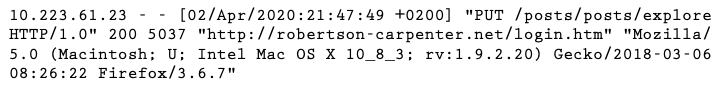
\includegraphics[scale=0.55]{images/apache-faker.png}
    \caption{Log-Output}
\end{figure}
\subsubsection{Zweck}
Die Überlegung zu diesem Generator war, den kompletten Prozess auf das Einfachste herunterzubrechen, um diesen realisierbar zu machen. Später sollte dieser dann in Phase-2 durch einen komplexeren selbst geschrieben Generator ersetzt werden.

\newpage
\subsection{Generator-Gerald}
\subsubsection{Allgemein}
Der Generator-Gerald ist das Modul, welches das Generieren der Zolldaten, wie in 3.2 Datenquellen erwähnt, implementiert und gehört somit zur Phase-2 des Prototyps. Der Generator ist in Kotlin auf Basis der JVM Plattform geschrieben und kann somit auf jedem System, welches das Java-Runtime-Environment installiert hat, laufen. Als Build-Automation-Tool kommt Gradle zum Einsatz, welches sich um die Ausführung der Unit-Tests und den Build-Prozess kümmert, welcher das ganze Programm und seine Dependencies in eine sogenannte Uber-JAR steckt. Dies sorgt dafür, dass das komplette Programm über eine einzige JAR ausführbar ist.
\vspace{5mm}\par
An erster Stelle der Designüberlegungen stand die Frage, auf Basis welcher Daten die Generierung erfolgen soll. Diese Überlegung wurde angeschnitten, um bei der Nutzung des Generators eine gewisse Variation und Bestimmung der generierten Daten zu ermöglichen. Somit wurden fünf Startparameter für den Generator definiert, welche in Form eines JSON-Strings übergeben werden müssen. Die dazu gehörige Datenklasse für die \textit{GenerationParams} sieht wie folgt aus:
\begin{lstlisting}[caption={GenerationParams}, language=Kotlin]
data class GenerationParams(
    val company: String,
    val plant: String,
    val importCountry: String,
    val periodRangeStart: Int,
    val periodRangeEnd: Int
)
\end{lstlisting}
\vspace{4mm}\par
Auf Basis dieser kann der Generator dann den folgenden Zolldeklarationsdatensatz erstellen.
Bei den generierten Daten gibt es vier Arten: 
\begin{itemize}
  \item \textbf{Parameterdaten}, diese werden beim Start des Programms übergeben und bleiben konstant bei jedem generierten Datensatz, auf diesen können Zufalls- und Zeitdaten basieren.
  \item \textbf{Zufallsdaten}, diese werden komplett zufällig unter speziellen Bedingungen, welche auch von anderen Zufallsdaten abhängen können, generiert.
  \item \textbf{Arraydaten}, über den Index wird ein Element aus einem Array ausgewählt.
  \item \textbf{Zeitdaten}, diese werden immer in Abhängigkeit von anderen Zeitdaten von einander generiert, die Parameterdaten zu Periode schränken dabei den Zeitraum ein, in welcher jene vorkommen dürfen.
\end{itemize}
\subsubsection{Verwendung des Generators}
Zum Start des Generators muss zwingend ein JSON-String mit dem \textit{GenerationParams} als erstes Startargument an das Programm übergeben werden. Hier die Namenserläuterungen:
\begin{itemize}
    \item \textit{company} - zweistelliger Kürzel der empfangenden Firma
    \item \textit{plant} - zweistelliger numerischer Code, welcher das Werk, in welches die Ware geliefert wird, identifiziert.
    \item \textit{importCountry} - Ländercode des Empfängerlandes nach ISO 3166-1 alpha 2
    \item \textit{periodRangeStart} - Zeitangabe des Jahres und Monats im Format YYYYMM, legt das erstmögliche Datum für die Generierung fest.
    \item \textit{periodRangeEnd} - Zeitangabe des Jahres und Monats im Format YYYYMM, legt das letztmögliche Datum für die Generierung fest.
\end{itemize}
Alle Parameter müssen gültig belegt werden, einzige Ausnahme bilden die zwei Parameter \textit{periodRangeStart}  und \textit{periodRangeEnd}. Diese können mit dem Wert 0 belegt werden, welcher dafür sorgt, dass intern \textit{periodRangeStart} auf den ersten Tag des aktuellen Jahres gesetzt wird und \textit{periodRangeEnd} auf den aktuellen Tag gesetzt wird.
\vspace{4mm}\par
Das zweite Startargument ist optional und bietet die Möglichkeit den Pfad zu definieren, in dem das Programm die JSON-File mit den generierten Daten ablegt. Dies sieht in der Praxis wie folgt aus:
\vspace{3mm}\par
\begin{lstlisting}[caption={Programmstart}]
java -jar generator-gerald.jar 
    "{  
        "company": "AR", 
        "plant": "77", 
        "importCountry": "DE", 
        "periodRangeStart": 201910,
        "periodRangeEnd": 201911
     }" 
    "/data/"
\end{lstlisting}
\vspace{4mm}\par
Das File wird hiermit unter Namen \textit{gen.json} im Pfad „/data/“ angelegt. Sollte sich bereits ein File mit diesem Namen vorfinden, wird dessen Inhalt überschrieben. Des Weiteren werden immer nur maximal 100 Datensätze generiert, wird diese Anzahl erreicht, werden die vorherigen Einträge überschrieben.

Auf Basis der Vorgaben sieht eine einziger genierter Zolldeklarationsdatensatz wie folgt aus:
\newpage
\begin{lstlisting}[caption={Ein generierter Datensatz} , language=Kotlin]
{
   "company":"CP",
   "plant":"01",
   "importCountry":"DE",
   "periodRangeStart":0,
   "periodRangeEnd":0,
   "declarationId":"UC5DJE",
   "shipmentId":"457L7D",
   "invoiceId":16905,
   "invoiceLineId":73,
   "status":"SDERR",
   "originCountry":"GB",
   "declarationDate":"2020-01-22",
   "customOffice":"DE2775",
   "customOfficeOfEntry":"DE2272",
   "declarant":"Dr. Leta Stamm",
   "localReference":"457L7D",
   "shipmentDate":"2020-05-05",
   "modeOfTransportAtTheBorder":"Truck",
   "modeOfTransportInland":"Truck",
   "containerized":true,
   "containerNumbers":"CO8408;CO0885;CO0867;CO4413;CO2539",
   "automationIndicator":"false",
   "exporterAddressNumber":"2550",
   "exporterAddress":"Brigadier Pumacahua, LINCE",
   "exporterRegistrationNumber":"471-7607",
   "exporterName":"Rhodes Furniture",
   "exporterRegion":"Lima",
   "exporterCountry":"PE",
   "importerAddressNumber":"62",
   "importerAddress":"Leobnerstrasse, 8042 GRAZ",
   "importerRegistrationNumber":"511-57180",
   "importerName":"RaseN",
   "importerRegion":"Styria",
   "importerCountry":"AT",
   "supplierAddressNumber":"81",
   "supplierAddress":"Bahnhofstrasse, 6850 DORNBIRN",
   "supplierRegistrationNumber":"781-03675",
   "supplierName":"Adaptas",
   "supplierRegion":"Vorarlberg",
   "supplierCountry":"AT",
   "invoiceLineFrightCosts":157.41,
   "invoiceLineInsuranceCosts":1.42,
   "invoiceLineAdditionalCosts":54.06,
   "invoiceLineGrossWeight":2809.77,
   "invoiceLineNetWeight":2675.97,
   "invoiceLineHSCode":"1441615055",
   "invoiceLineValue":5246.99,
   "invoiceLineQuantity":1420,
   "invoiceLineCustomValue":5301.05,
   "invoiceLineVAT":0.0,
   "invoiceLineDuties":848.17,
   "invoiceLinePreferentialCode":"non-preferential: 142",
   "invoiceLineLastModified":"2020-01-26",
   "invoiceLastModified":"2020-01-30",
   "shipmentLastModified":"2020-02-09",
   "declarationLastModified":"2020-02-03"
}
\end{lstlisting}
\subsubsection{JSON-Serialisierung}
Die JSON-Serialisierung läuft mittels der Kotlin-Multiplattform-Library kotlinx.serialization ab. Standardmäßig kann diese die Kotlin-Datentypen serialisieren, für andere muss ein eigener Serializer geschrieben werden. Beide Varianten werden vom Generator-Gerald verwendet.
\vspace{4mm}\par
Die Serialisierung der GenerationParams erfolgt über die Standardmäßige, da dieses Objekt auf den Kotlin-Datentypen  \textit{String} und  \textit{Int} basiert. Die Nutzung sieht im Code wie folgt aus:
\begin{lstlisting}[caption={GenerationParams Datenklasse} , language=Kotlin]
@Serializable
data class GenerationParams(...) {...}
...
val jsonSerializer = Json(JsonConfiguration.Stable)
generationParams = jsonSerializer.parse(
    GenerationParams.serializer(), args[0])
\end{lstlisting}
\vspace{4mm}\par
Wie zu sehen ist, reicht eine Annotation zur Verwendung vollkommen aus. \textit{Args[0]} beschreibt hier den JSON-String, welcher bei Start des Programms übergeben wird.
\vspace{4mm}\par
\newpage
Anderst sieht die Sache bei der Serialisierung der \textit{GeneratedData} aus. In diesem Objekt werden auch Nicht-Kotlin-Datentypen verwendet, wie etwa \textit{Date} aus der java.util-Library. Dies wird durch die Tatsache begründet, dass es keinen nativen Kotlin-Datentyp für das Abspeichern eines Datums gibt und somit auf eine Java-Library ausgewichen werden muss. Vor der Nutzung muss also ein Serializer für die Typ \textit{Date} geschrieben werden, dies sieht wie folgt aus:
\begin{lstlisting}[caption={Custom Serializer} , language=Kotlin]
@Serializer(forClass = Date::class)
object DateSerializer: KSerializer<Date> {
    private val dateFormat: DateFormat = SimpleDateFormat("yyyy-MM-dd")

    override val descriptor: SerialDescriptor =
        StringDescriptor.withName("WhitCustomDefault")

    override fun deserialize(decoder: Decoder): Date {
        return dateFormat.parse(decoder.decodeString())
    }

    override fun serialize(encoder: Encoder, obj: Date) {
        encoder.encodeString(dateFormat.format(obj))
    }
}
\end{lstlisting}
\vspace{4mm}\par
Somit weiß der Serializer mithilfe von  \textit{DateFormat}, wie er die Daten zu deserialisieren beziehungsweise zu serialisieren hat.

\subsubsection{Country-Klasse}
Ein \textit{Country} besteht aus folgenden zwei Elementen, einem Code-Feld, dies entspricht dem Ländercode, und einem Namen. Diese Klassen dienen dazu, den Ländercode, welcher in den Startparametern mitgegeben wird, auf die Echtheit zu validieren. Um eine Vergleichsliste zu erhalten, wird die \textit{Locale}-Klasse aus der java.utils-Library verwendet.
\newpage
Die \textit{loadCountries}-Funktion  sieht damit so aus:
\begin{lstlisting}[caption={ISO-Länder laden} , language=Kotlin]
private fun loadCountries(): List<Country> {
    val countries = mutableListOf<Country>()

    Locale.getISOCountries().forEach {
        val iso = it;
        val locale = Locale("", iso)
        countries.add(Country(iso, locale.displayCountry))
    }

    return countries
}
\end{lstlisting}
\vspace{4mm}\par

\subsubsection{DateMaker-Funktionen}
Diese Sammlung an Funktionen dient dazu, die Operationen mit \textit{Date}-Objekten abzudecken.
\begin{lstlisting}[caption={String-Daten parsen} , language=Kotlin]
fun String.toDate(): Date {
    var result = Date()
    val dateRegex: Regex = 
        """([12]\d{3}-(0[1-9]|1[0-2])-(0[1-9]|[12]\d|3[01]))"""
        .toRegex()

    if (dateRegex matches this) {
        try {
            val dateFormat = SimpleDateFormat("yyyy-MM-dd")
            result = dateFormat.parse(this)
        } catch (e: Exception) {
            e.printStackTrace()
        }
    }
    return result
}
\end{lstlisting}
\vspace{4mm}\par
Diese Extension-Funktion ist das Herzstück der Sammlung und erlaubt es mittels Validierung über eine Regular-Expression den String als valide zu kennzeichnen, so dass dieser in ein \textit{Date}-Objekt konvertiert werden kann.
\begin{lstlisting}[caption={Daten generieren} , language=Kotlin]
fun makeRandomDateWithinRange(minDate: Date, maxDate: Date): Date {
    var randomDate = Date()
    if (minDate.time < maxDate.time) {
        randomDate = Date(ThreadLocalRandom.current()
        .nextLong(minDate.time, maxDate.time))
    }
    return randomDate
}
\end{lstlisting}
\vspace{4mm}\par
Durch diese Funktion werden alle zufälligen \textit{Date}-Objekte generiert, da diese immer nur in einem bestimmten Zeitraum vorkommen dürfen, um ein logisches Zusammenspiel der einzelnen Zeitmarken zu erhalten.

\subsubsection{InvoiceLine-Klasse}
Ein \textit{InvoiceLine}-Datensatz wird durch einen \textit{InvoiceLineGenerator} erstellt. Eine solches \textit{InvoiceLine}-Element ist wie folgt aufgebaut:
\begin{lstlisting}[caption={Rechnungszeile} , language=Kotlin]
data class InvoiceLine(
    val frightCosts: Float,
    val insuranceCosts: Float,
    val additionalCosts: Float,
    val grossWeight: Float,
    val netWeight: Float,
    val hsCode: String,
    val value: Float,
    val quantity: Int,
    val customValue: Float,
    val vat: Float,
    val duties: Float,
    val preferentialCode: String,
    val lastModified: Date
)
\end{lstlisting}
\vspace{4mm}\par
\newpage
Und die Folgenden sind die Parameter welcher der \textit{InvoiceLineGenerator} verwendet um alle diese Daten zu generieren: 

\begin{lstlisting}[caption={Rechnungsparamter} , language=Kotlin]
class InvoiceLineGenerator(
    private val shipmentDate: Date,
    private val minDate: Date,
    private val todayDate: Date,
    private val sent: Boolean
) {...}
\end{lstlisting}
\vspace{4mm}\par
Alle Zahlenwerte im \textit{InvoiceLineGenerator} sind Zufallsdaten, welche auf dem Wert der Variable \textit{value}, welche zufällig generiert wird, basieren. Hier ein Beispiel:
\begin{lstlisting}[caption={Versandkosten generieren} , language=Kotlin]
private fun genFrightCosts(): Float {
    val percentageOfNetValue = (1..5).random().toFloat() / 100
    return (value * percentageOfNetValue).round(2)
}
\end{lstlisting}
\vspace{4mm}\par
Die Versandkosten, welche wiederum Ausgangsbasis für weitere Werte sind, basieren zu einem Teil auf dem Wert \textit{value} und einer weiteren zufallsgenerierten Komponente.
\vspace{4mm}\par
Für \textit{preferentialCode} wurde wiederum das Konzept der Arraydaten verwendet:
\begin{lstlisting}[caption={Preferenzcodebasis} , language=Kotlin]
val POSSIBLE_PREFERENTIAL_CODES = arrayOf(
    "preferential: 103",
    "non-preferential: 142"
)
\end{lstlisting}
\vspace{4mm}\par
Wie ersichtlich gibt es für die generierten Zolldeklarationen nur zwei Möglichkeiten, die zufällige Auswahl erfolgt dann über diese Funktion:
\begin{lstlisting}[caption={Preferenzcodegenerierung} , language=Kotlin]
private fun genPreferentialCode(): String {
    val randomIndex = (POSSIBLE_PREFERENTIAL_CODES.indices).random()
    return POSSIBLE_PREFERENTIAL_CODES[randomIndex]
}
\end{lstlisting}
\newpage
Da sich das Datum der letzen Modifizierung der Rechnungsstelle mit den andern Zeitmarkern im Einklang befinden soll, werden hierfür die Parameterwerte der Daten dafür verwendet das neue Datum zu generieren. Aus diesem Grund ist die Abfolge der zu generierenden Daten vor allem bei den Zeitmarken von essenzieller Bedeutung, um sinnenhafte Daten erstellen zu können.
\begin{lstlisting}[caption={Änderungsdatum generieren} , language=Kotlin]
private fun genLastModified(): Date {
    val minDate = minDate
    val maxDate = if (sent) { shipmentDate } else { todayDate }
    return makeRandomDateWithinRange(minDate, maxDate)
}
\end{lstlisting}
\vspace{4mm}\par
\subsubsection{Participant-Klasse }
Zu einem \textit{Participant} gehören sowohl Exporteure, Importeure als auch Lieferanten. Sie alle teilen die gleiche Datenstruktur, welche wie folgt aussieht:
\begin{lstlisting}[caption={Participant-Datenklasse} , language=Kotlin]
data class Participant(
    val addressNumber: String,
    val address: String,
    val registrationNumber: String,
    val name: String,
    val region: String,
    val country: String
)
\end{lstlisting}
\vspace{4mm}\par
Bei dieser Klasse wird die Generierungsart Arraydaten angewandt, dies bedeutet, dass bereits vorliegende Datensätze in einem Array existieren und nur noch über einen zufälligen Index ausgewählt werden. Eine solches Arrayelement sieht wie folgt aus:
\begin{lstlisting}[caption={Generierter Participant} , language=Kotlin]
Participant(
    "bld. 30",
    "Lidonu, RIGA",
    "46-19-96",
    "Complete Tech",
    "Riga",
    "LV"),
\end{lstlisting}
\vspace{4mm}\par
\subsubsection{Generate-Companion-Objekt}
Weitere Arraydaten werden für die möglichen Status der Sendung verwendet, da es sich bei diesen um fixe Werte handelt, welche eine Sendung annehmen kann. Auch werden die Transportmöglichkeiten mittels eines Array angegeben, da beim Zollwesen nur zwischen vier Möglichkeiten unterschieden wird: 
\begin{lstlisting}[caption={Transportmöglichkeiten} , language=Kotlin]
val MODES_OF_TRANSPORT = arrayOf(
    "Train",
    "Ship",
    "Airplane",
    "Truck"
)
\end{lstlisting}
\vspace{4mm}\par
\subsubsection{Generate-Klasse}
Neben der \textit{InvoiceLineGenerator}-Klasse handelt es sich bei \textit{Generate} um die zweite wichtige Generierungsklasse. Die Überlegung der Trennung dieser zwei Teile beruht darauf, dass die \textit{InvoiceLine}-Klasse die tiefste Ebene der Zolldatendeklaration abbildet und die \textit{Generate}-Klasse hingegen die oberen Ebenen, welche als Basis für die \textit{InvoiceLine} benötigt werden. 
\vspace{4mm}\par
Das Datum aus der InvoiceLine wird danach wiederum für die Evaluierung verwendet  wann die letze Veränderung in der Deklaration stattgefunden hat. Dies würde in dem Fall vorliegen, dass das Datum aus der InvoiceLine nach dem aktuell gesetzten Deklarationsdatum liegen würde:
\begin{lstlisting}[caption={Deklarationsveränderung generieren} , language=Kotlin]
fun genDeclarationLastModified(): Date {
    val minDate = if (invoiceLastModified < declarationDate ) 
        { declarationDate } 
    else { invoiceLastModified }
    val maxDate =  if (sent) { shipmentDate } else { todayDate }
    return makeRandomDateWithinRange(minDate, maxDate)
}
\end{lstlisting}
\vspace{4mm}\par
\newpage
Einer der wichtigsten Bestandteile dieser \textit{Generate}-Klasse ist der Sendestatus, denn er bestimmt, ob eine Sendung schon auf dem Weg ist beziehungsweise war und somit danach nicht mehr bearbeitet werden kann. Die Generierung des Sendestatus erfolgt über folgendes Array:
\begin{lstlisting}[caption={Mögliche Status} , language=Kotlin]
val POSSIBLE_STATUS = arrayOf(
    "CLOSED",
    "DACC",
    "DEACT",
    "DERR",
    "DESENT",
    "DSENT",
    "NDERR",
    "NDFB",
    "NDSENT",
    "OPEN",
    "SDERR")
...
private val sent = SENT_STATUS.contains(status)
\end{lstlisting}
\vspace{4mm}\par
Wurde also ein gesendeter Status ausgewählt, so wird das \textit{maxDate} der Zeitmarken-Generierungen auf das \textit{shipmentDate} gesetzt.

\subsubsection{Main-File}
\begin{lstlisting}[caption={} , language=Kotlin]
val genData = generateDataItem(generationParams)
...
val jsonGenData = jsonSerializer.stringify(
    GeneratedData.serializer(), 
    genData)
...
buildJsonFile(jsonGenData)
\end{lstlisting}
\vspace{4mm}\par
In der \textit{main-Funktion} wird der Datensatz der \textit{generateDataItem}-Funktion, welche als Verbindungsstück zur \textit{Generate-Klasse} agiert, dann wieder wie folgt in ein JSON umgewandelt und anschließend an die \textit{buildJsonFile}-Funktion abgegeben, um je nach Datensatzanzahl die Datei anzulegen, zu überschreiben oder weiter zu schreiben. 

\subsection{Automatisierte Unit-Tests durch GitHub-Actions}
\begin{figure}[H]
    \centering
    
\includegraphics[scale=0.2]{images/github-actions.png}
    \caption{GitHub Actions (02.04.2020)}
    \label{img:}
    \url{https://github.blog/wp-content/uploads/2019/08/DL-V2-LinkedIn_FB.png?w=1200}
\end{figure}
Mithilfe von GitHub Actions können sogenannte Workflows erstellt werden. Im Fall vom Generator-Gerald sorgt ein Action-Workflow dafür, dass bei jedem push- oder pull-request auf dem Master automatisiert mittels Gradle sofort Feedback zur Funktionalität der aktuellen Änderung gegeben wird. Geschrieben werden diese Workflows mittels einer YAML-File. Der für die Ausführung der Unit-Tests verantwortliche YAML-Code sieht wie folgt aus:
\begin{lstlisting}[caption={Gradle Unit-Test Action}]
# Display name of the action
name: Gradle-Tests
# Defines when the action should run
on:
    push:
      branches: [ master ]
    pull_request:
      branches: [ master ]
# Definition of what should be done
jobs:
  gradle:
    runs-on: ubuntu-latest # The task should be executed on an ubuntu env.
    steps:
      - uses: actions/checkout@v1
      - uses: actions/setup-java@v1
        with:
          java-version: 11
      - uses: eskatos/gradle-command-action@v1
        with:
          build-root-directory: extract-transform/generator-gerald
          wrapper-directory: extract-transform/generator-gerald
          arguments: test
\end{lstlisting}
\vspace{4mm}\par
 Zu aller erst  wird definiert, welche Aktionen diesen Workflow aktivieren sollen. Wie bereits erwähnt, wird dieser nur bei Master-Aktionen ausgeführt. In \textit{jobs} definieren wir, auf welchem System dieser Workflow laufen soll. Um Gradle verwenden zu können, wird zusätzlich noch Java benötigt, dies erfolgt mittels \textit{actions/setup-java@v1}. Nun kann mittels der \textit{gradle-command-action} der Unit-Test für das entsprechende Verzeichnis erfolgen.
 Wird der Unit-Test nicht erfolgreich abgeschlossen, erhalten wir eine visuelle Meldung zu unserem Commit:
\begin{figure}[H]
    \centering
    
\includegraphics[scale=1]{images/github-action-error.png}
    \caption{Fehlermeldung beim Commit (02.04.2020)}
\end{figure}
Sollen genauere Information zum Fehlschlagen des Commits erhalten werden, kann dies über den Action-Reiter getan werden.
\begin{figure}[H]
    \centering
    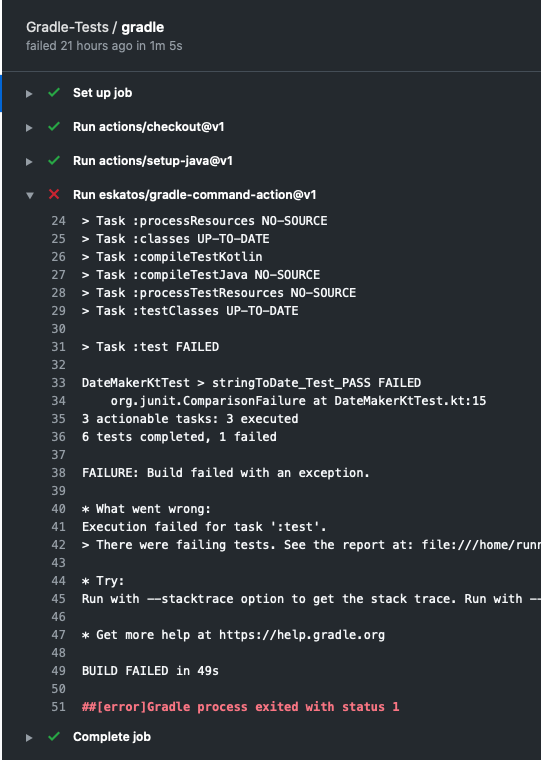
\includegraphics[scale=0.5]{images/github-action-detail-error.png}
    \caption{Action-Detailansicht (02.04.2020)}
\end{figure}
So kann jetzt entnommen werden, welcher Test genau fehlschlug. Da es sich um den komplett identischen Unit-Test, wie auf dem lokalen Gradle-Projekt, handelt, kann sofort der Fehler auch auf dem lokalen System reproduziert werden, sofern sich dieses auf dem aktuellen Stand des Masters befindet. 
